%-------------------------------------------------------------
\title[C2C compiler]{Analyse de pointeurs avec LLVM}
%\vspace{-1cm}


\titlegraphic{
\vspace{3mm}

\includegraphics[height=35pt]{logo_lip}
\hspace{3cm}

\includegraphics[height=45pt]{logo_lyon1}
\hspace{3mm}

}

\author[Aurélien Chemier]{Aurélien Chemier}
   
\institute[LIP]{Laboratoire de l'Informatique du Parallélisme (ENS Lyon)}
\date[Janvier-Février 2014]{MIF20}


%-------------------------------------------------------------
\begin{document}
%\addtocounter{framenumber}{-1} 

\begin{frame}[plain]
   \titlepage

{\scriptsize Advised by Laure Gonnord. 
}
 \end{frame}

\begin{frame}[plain]
	\tableofcontents
\end{frame}

\section{Contexte de recherche et problématique}

\begin{frame}\frametitle{contexte d'équipe}

\begin{itemize}
  \item COMPSYS est une équipe-projet de recherche 
    \begin{itemize}
    \item Inria 
    \item Laboratoire de l'Informatique du Parallélisme (LIP).
    \item Localisée à l'Ecole Normale Supérieure de Lyon (ENS Lyon).
    \end{itemize}
  
  
  \item L'objectif de Compsys:
    \begin{itemize}
    \item développement de techniques de compilation.
    \item optimisations de codes.
    \item pour systèmes embarqués de calcul.
    \end{itemize}

  \end{itemize}

\end{frame}


\begin{frame}\frametitle{Présentation du sujet}
  \begin{itemize}

  \item L'objectif du TER 
    \begin{itemize}
    \item optimisation d'un code C.
    \item optimisations des pointeurs.
    \end{itemize}
  \item optimisations déjà existantes: (modèle polyédrique)
  \item parallelisation des boucles imbriquées.
  \end{itemize}

\end{frame}

\begin{frame}
  Par exemple pour un code donné:
  \begin{center}
     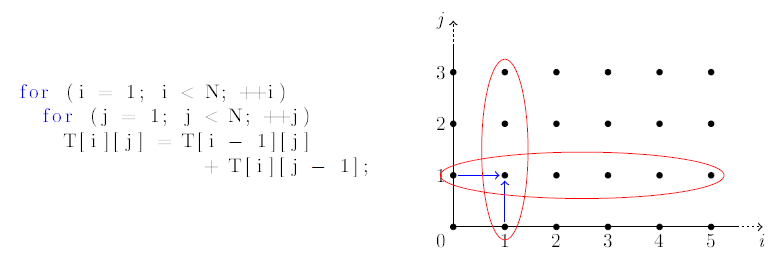
\includegraphics[scale=0.4]{poly.png}
  \end{center}
  On obtient : 
  \begin{center}
     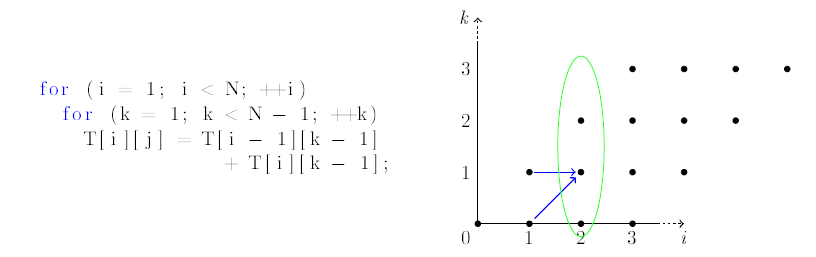
\includegraphics[scale=0.4]{polyok.png}
  \end{center}


\end{frame}

\begin{frame}\frametitle{Limitations}

  \begin{itemize}

  \item Actuellement, le modèle polyédrique = tableau statique.
  \item Les optimisations sur les pointeurs = peu nombreuses.

  \end{itemize}
\end{frame}


\section{Contexte technologique} %%% Aurélien seulement 

\begin{frame}
  \begin{itemize}

  \item LLVM 
  \begin{itemize}
  \item Infrastructure de compilateur.
  \item Représentation intermédiaire du code.
  \item Optimisation d’un programme à tous les niveaux.
  \end{itemize}
  
  \item Clang 
  \begin{itemize}
  \item Front-end de LLVM
  \item Analyses lexicales et syntaxiques.
  \item Arbre  de syntaxe abstraite et graphe de controle de flot
  \item Conversion en code intermediaire.
  \end{itemize}
  
  \item gratuit et open source (3.4 stable, 3.5 en developpement).
  \end{itemize}
\end{frame}


\begin{frame}
	CFG (Control flow graph): graphe de tous les chemins suivis par un programme durant son exécution. 
	 \begin{center}
     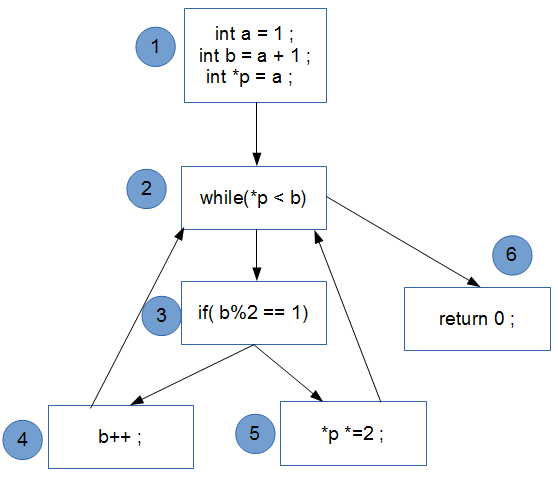
\includegraphics[scale=0.4]{CFG.png}
  \end{center}
\end{frame}

\begin{frame}
  Lors de son Stage, Christophe Baccara a créé plusieurs outils permettant d'étudier les propriétés des pointeurs.
  \begin{itemize}
  \item Création du CFG du programme.
  \item Controle des pointeurs constants.
  \item Etudes des alias de pointeurs.
  \item Réécriture d'un code.
  \end{itemize}
\end{frame}

\begin{frame}\frametitle{Exemple: pointeurs constants}
  \label{exemple}
  Dans le cas du code suivant :
  \lstinputlisting[language=C,frame=single,firstline=2, lastline=8]{Exemple/pointeurConstant.c}
  Le travail de C. Baccara permet d'avoir le résultat suivant:
  \begin{center}
     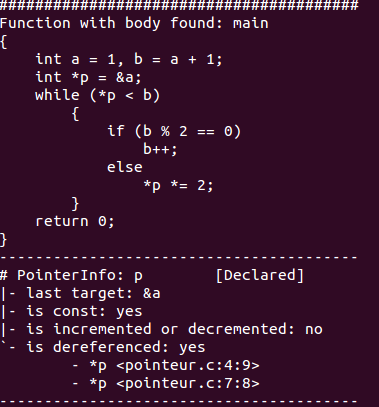
\includegraphics[scale=0.25]{ptrconstant.png}
 \end{center}
\end{frame}


\section{Transformation sur les pointeurs}%%% aurélien

\begin{frame}\frametitle{pointeurs constants}
  Reprenons le code précédent:
  \lstinputlisting[language=C,frame=single,firstline=2, lastline=8]{Exemple/pointeurConstant.c}
  L'objectif  :
  \begin{enumerate}
  \item Créer le CFG du programme.
  \item Trouver les pointeurs constants dans le CFG.
  \item Réécrire le CFG sans les pointeurs constants du code.
  \end{enumerate}
\end{frame}

\begin{frame}
  \`A la fin :
  \lstinputlisting[language=C,frame=single,firstline=2, lastline=8]{Exemple/pointeurConstantOpt.c}
  Le pointeur a été enlevé.
\end{frame}

\begin{frame}\frametitle{tableaux}
  Un algorithme de tri sur un tableau dynamique
  \lstinputlisting[language=C,frame=single,firstline=6, lastline=18]{Exemple/malloc.c}
\end{frame}
   
\begin{frame}
  L'objectif :
  \begin{enumerate}
  \item Créer le CFG du programme.
  \item Trouver l'allocation du tableau dans le CFG.
  \item Controler que la taille du tableau est constante.
  \item Réécrire le CFG en remplaçant le tableau dynamique par un tableau statique.
  \end{enumerate}
\end{frame}

\begin{frame}\frametitle{tableaux}
  \`A la fin :
  \lstinputlisting[language=C,frame=single,firstline=6, lastline=18]{Exemple/mallocOpt.c}
\end{frame}

\section{Résultats}%% aurélien

\begin{frame}
  Le travail que j'ai fait a principalement porté sur les alias de pointeurs constants (diapo \ref{exemple}).
  
  Actuellement, le compilateur trouve : 
  \begin{itemize}
  \item Les pointeurs à remplacer.
  \item Où les remplacer.
  \item Par qui les remplacer.
  \end{itemize}
\end{frame}
%%%%%%%%%%%%%%%%%%%%%%%%%%%%%%% fin aurélien seulement

\section{Conclusion}
\begin{frame}

  Beaucoup à faire dans l'optimisation des pointeurs.
  
  Actuellement:
  \begin{itemize}
  \item Détection des alias de pointeurs.
  \end{itemize}
\end{frame}

\begin{frame}
  Travail à faire:
  \begin{itemize}
  \item Modification ou suppression des alias
  \item C
ontrole des tableaux.
  \end{itemize}
  
\end{frame}
